\documentclass[12pt]{article}
\usepackage[margin=1in]{geometry}
\usepackage{amsmath}
\usepackage{amsfonts}
\usepackage{tikz}
\usepackage{graphicx}
\usepackage{hyperref}

\begin{document}

\title{Bohr \& Rutherford}
\author{Nathan Solomon}
\maketitle

This week's notes is a whole hodgepodge of experiments and new ideas from the early 1900s.

\section{Miscellaneuous Experiments (in no particular order)}
\begin{itemize}
    \item J.J. Thomson figures out that cathode rays are made of electrons
    \item Thomson measures charge-to-mass ratio of electron by using a velocity selector
    \item Fletcher \& Millikan's oil drop experiment determines the quantized unit of electric charge
    \item Michael Faraday discovers his law of electrolysis
    \item Rutherford shows that positive charge is concentrated at tiny centers of atoms
    \item Kirchhoff realizes that the emissivity and the absorptivity of a material are the same. He also explains Fraunhofer D-lines.
    \item Bunsen uses absorption spectra of the sun to show what elements are present on its surface
    \item Balmer comes up with experimental formula for wavelengths of emission lines of hydrogen
    \item Bohr proposes electrons orbit in ``stationary states", which don't follow classical rules for Bremsstrahlung
    \item Franck \& Hertz show that when electrons are fired through mercury vapor, the amount of energy they lose can only be an integer multiple of 4.9 eV, which confirms Bohr's atomic model
\end{itemize}

\section{Bohr's Model}
Bohr proposed that the orbital angular momentum of an electron can only be an integer multiple of the reduced Planck constant:
\[ L := m_e v r \in \hbar \mathbb{N} \]
In the Bohr model, whenever an atom absorbs or emits a photon, the frequency of that photon is unrelated to the frequency of the electron's orbit, which makes no sense if you think of it in terms of classical physics.

For a hydrogen atom, the centripetal force on an electron is
\[ F = \frac{m_e v^2}{r} = \frac{ke^2}{r^2} \]
where $k := 1 / (4 \pi \varepsilon_0)$. From that, you can use more classical physics to get the potential energy ($U$), kinetic energy ($K$), and total energy ($E$) of the electron.
\[ U =  - \frac{k e^2}{r} , K = \frac{k e^2}{2 r} , E = - \frac{k e^2}{2 r} \]
You can now solve for the velocity:
\[ v = r^2 F / L = \frac{k e^2}{n \hbar} \hspace{1cm} \forall n \in \mathbb{N}\]
And the radius:
\[ r = \frac{n \hbar}{m_e v} = \frac{n^2 \hbar^2}{m_e k e^2} \hspace{1cm} \forall n \in \mathbb{N} \]
That quantity when $n=1$ is called the Bohr radius, $a_0$
\[ a_0 := \frac{\hbar^2}{m_e k e^2} = \frac{h^2 \varepsilon_0}{\pi m_e e^2} \approx .5292 \text{\AA} \]

\section{Rutherford Scattering}
If you fire a beam of $\alpha$ particles at a perpendicular sheet of gold foil, you might expect them to go right through, and most do, but some will be scattered. The number of particles you'll detect that are scattered at an angle $\phi$ is
\[ \Delta n = \frac{k^2 Z^2 e^4 N n A}{4 R^2 E^2 \sin^4 (\phi / 2)} \]
where $k$ is Coulomb's constant, $Z$ is the atomic number of the metal, $N$ is the number of nuclei per unit area, $n$ is the number of $\alpha$ particles fired per unit time, $A$ is the area of the detector, $R$ is the distance from the detector to the point where $\alpha$ particles hit the foil, and $E$ is the kinetic energy of each $\alpha$ particle.

We do not need to know the derivation of that formula, only that it comes from electrostatic repulsions between the metal nuclei and the $\alpha$ particles. If the $\alpha$ particles are moving fast enough, they will actually touch the surface of the nuclei, and that equation will stop working.

\section{Compton Scattering}
To make this derivation extra fun, we'll use 4-momentum. Normally that means using the Minkowski product, but I don't like that -- I prefer to just make the time component of 4-momentum imaginary, which has the same effect as using a (-1, 1, 1, 1) metric signature.
\[ \boldsymbol{p} := \begin{bmatrix}
    iE/c \\
    p_x \\
    p_y \\
    p_z
\end{bmatrix} \]
This works out nice because $\boldsymbol{p}^2 = p^2 - E^2/c^2 = p^2 - (p^2 c^2 + m_0^2 c^4) / c^2 = - m_0^2 c^2$ which means that $\boldsymbol{p}$ is Lorentz invariant.

Compton scattering describes a photon colliding with an electron. Suppose the  electrons starts at rest, and a photon is moving right (in the +x direction towards it). After colliding, the electron is moving up and to the right, at an angle $\theta$ above the horizontal, and the photon is moving down and to the right, at an angle $\phi$ below the horizontal. We want to be able to find how much the wavelength of the photon changes, given the angle $\theta$.

\begin{figure}[h]
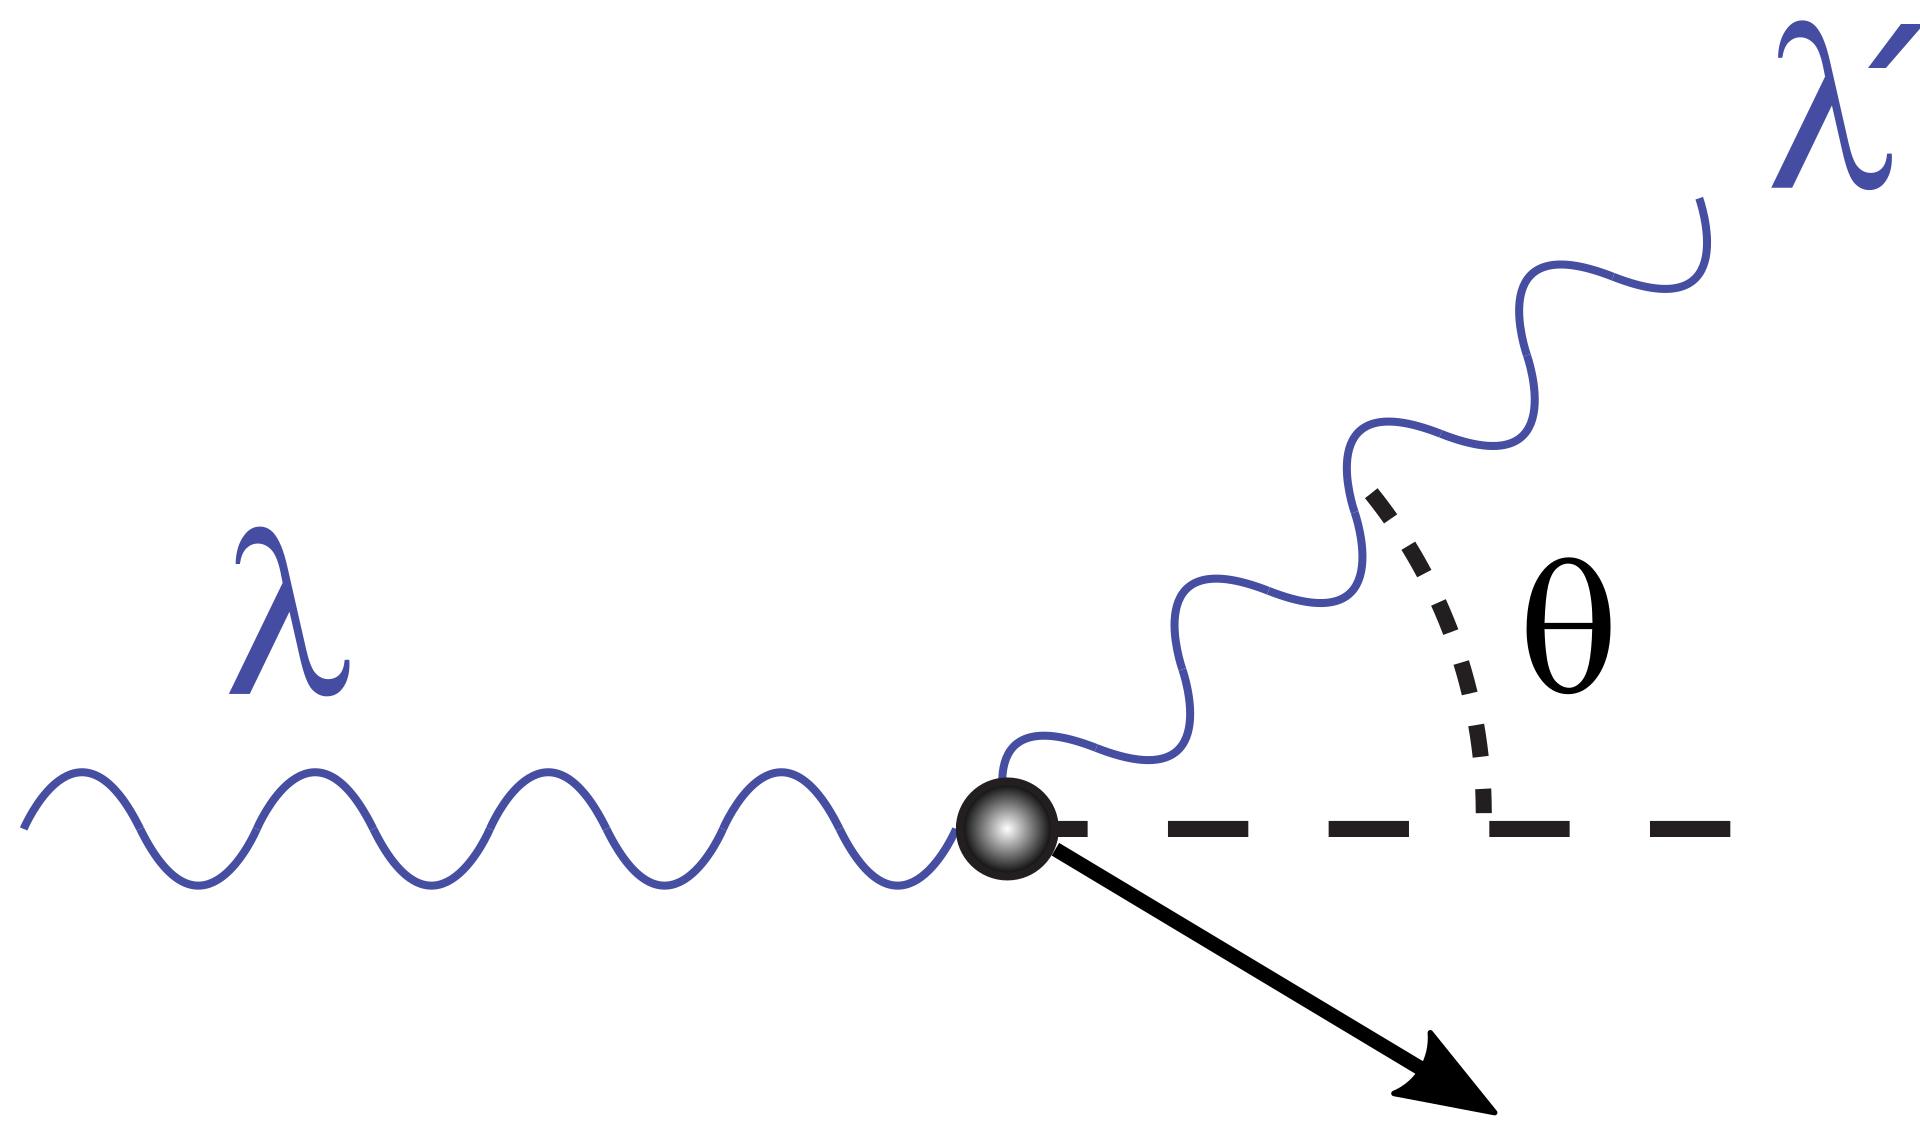
\includegraphics[width=8cm]{Compton-scattering.png}
\centering

By JabberWok, CC BY-SA 3.0, \url{https://commons.wikimedia.org/w/index.php?curid=2078004}
\end{figure}
Now we can use the conservation of 4-momentum to solve for $\lambda' - \lambda$
\[ \boldsymbol{p_\gamma} + \boldsymbol{p_e} = \boldsymbol{p_\gamma '} + \boldsymbol{p_e '} \]
Next, substitute in the definition of 4-momentum, and the fomulas for momentum and energy of a photon
\[ \begin{bmatrix} i h / \lambda \\ h / \lambda \\ 0 \\ 0 \end{bmatrix}
+ \begin{bmatrix} i m_e c \\ 0 \\ 0 \\ 0 \end{bmatrix}
= \begin{bmatrix} i h / \lambda' \\ (h / \lambda') \cos \theta \\ (h / \lambda') \sin \theta \\ 0 \end{bmatrix}
+ \boldsymbol{p_e '} \]
Since the electron does not gain or lose mass, the norm of its 4-momentum doesn't change, so
\[ \left( \begin{bmatrix} i h / \lambda \\ h / \lambda \\ 0 \\ 0 \end{bmatrix}
+ \begin{bmatrix} i m_e c \\ 0 \\ 0 \\ 0 \end{bmatrix}
- \begin{bmatrix} i h / \lambda' \\ (h / \lambda') \cos \theta \\ (h / \lambda') \sin \theta \\ 0 \end{bmatrix} \right)^2
= (\boldsymbol{p_e'})^2 = (\boldsymbol{p_e})^2 = - m_e^2 c^2 \]
The left hand side of that equation simplifies to
\begin{align*}
    - m_e^2 c^2 &= \begin{bmatrix} i h / \lambda + i m_e c - i h / \lambda' \\ h / \lambda - (h / \lambda') \cos \theta \\ - (h / \lambda') \sin \theta \\ 0 \end{bmatrix}^2 \\
                &= (ih/\lambda + im_ec - ih/\lambda')^2 + (h/\lambda - h\cos \theta / \lambda')^2 + (-h \sin \theta / \lambda')^2 \\
                &= - m_e^2c^2 - 2hm_ec/\lambda + 2h^2/(\lambda' \lambda) + 2hm_ec/\lambda' - 2h^2\cos \theta / (\lambda' \lambda)
\end{align*}
Now all you have to do is manipulate that equation a bit more
\begin{align*}
    - m_e^2 c^2 &= - m_e^2c^2 - 2hm_ec/\lambda + 2h^2/(\lambda' \lambda) + 2hm_ec/\lambda' - 2h^2\cos \theta / (\lambda' \lambda) \\
    0 &= - 2m_ec/\lambda + 2h/(\lambda' \lambda) + 2m_ec/\lambda' - 2h\cos \theta / (\lambda' \lambda) \\
    0 &= -m_ec\lambda' + h + m_ec\lambda - h\cos \theta \\
    \lambda' - \lambda &= \frac{h}{m_e c} (1 - \cos \theta) = \lambda_C (1 - \cos \theta)
\end{align*}
That last equation is the formula for Compton scattering. The Compton wavelength of a particle with mass $m$ is a useful constant, defined as $\lambda_C := h/(m c)$.

\end{document}
